% A simple LaTeX template for lab reports in TDT4258 Energy Efficient Computer Design
% by Yaman Umuroglu (yamanu@idi.ntnu.no)
% Feel free to customize the style as you see fit, but the chapters/sections mentioned in the
% template should be included with the appropriate content.

\documentclass[abstract=on]{scrreprt}
\usepackage[utf8]{inputenc}


\usepackage{natbib}
\usepackage{graphicx}
\usepackage{listings}
\usepackage{color}
 
\definecolor{codegreen}{rgb}{0,0.6,0}
\definecolor{codegray}{rgb}{0.5,0.5,0.5}
\definecolor{codepurple}{rgb}{0.58,0,0.82}
\definecolor{backcolour}{rgb}{0.95,0.95,0.92}
 
\lstdefinestyle{mystyle}{
    backgroundcolor=\color{backcolour},   
    commentstyle=\color{codegreen},
    keywordstyle=\color{magenta},
    numberstyle=\tiny\color{codegray},
    stringstyle=\color{codepurple},
    basicstyle=\footnotesize,
    breakatwhitespace=false,         
    breaklines=true,                 
    captionpos=b,                    
    keepspaces=true,                 
    numbers=left,                    
    numbersep=5pt,                  
    showspaces=false,                
    showstringspaces=false,
    showtabs=false,                  
    tabsize=2
}
 
\lstset{style=mystyle}

% Edit the meta.tex file to change title, group number and author names
% Fill in the report title, group number and student names here
\newcommand{\mytitle}{Exercise 3}
\newcommand{\mygroupnumber}{12}
\newcommand{\myauthor}{Håvard Pettersson\\Hans-Kristian Bruvold\\Ole Morten Saggau}

\title{\mytitle}
\author{\myauthor}
\date{\today}



\begin{document}
% The title page, edit if you want to customize it
\begin{titlepage}

\includegraphics[height=1.5cm]{images/ntnu_logo.pdf}\\[1cm]   
\begin{center}

 
% Upper part of the page
~\\[1.5cm]

\textsc{\Large TDT4258 Energy Efficient Computer Design\\Laboratory Report}\\[0.5cm]

% Set the title of the Document between two horizontal lines
\hrule ~\\[0.2cm]
{\huge \bfseries \mytitle}\\[0.4cm]		% print the title of the document
\hrule ~\\[1.5cm]

% Additional Information about the document
\begin{minipage}{0.4\textwidth}
    \centering
	\large
		\emph{Group \mygroupnumber:}\\~\\
		\myauthor
\end{minipage}

\vfill

% Bottom of the page
{\large \today}

\end{center}
\end{titlepage}


% Main matter - edit corresponding file under content/ to change
\begin{abstract}
This report introduces assembly programming for the EFM32GG-DK3750 development board, including interrupt handling, GPIO and energy optimizations. The goal of the exercise was to implement a simple interaction between buttons and LEDs on a gamepad  using the GPIO pins on the development board. The assembly code was built and debugged using the GNU toolchain, and flashed and profiled using the eACommander and eAProfiler programs.

A solution where each button on the gamepad maps to a separate LED was implemented. Energy efficiency was achieved by using GPIO interrupts for the buttons (as opposed to polling) and by enabling sleep mode on the microcontroller.
\end{abstract}
\tableofcontents %do not remove this
\chapter{Introduction}
Energy efficiency is very important in embedded systems development. Often, the microcontroller and its peripherals are battery-powered, or are similarly constrained. For this reason, one has to be careful when implementing programs for such microcontrollers. 

Our goal is to implement a program for the Cortex-M3 microcontroller on the EFM32GG-DK3750 development board that interfaces with an external gamepad using GPIO, and improving the energy efficiency of this implementation as much as possible. The gamepad has eight buttons and eight LED lights, and the implementation should make button presses light up the LEDs in some way.
\chapter{Background and Theory}
%This chapter should describe the theoretical background needed to understand and solve the problem. 
%For instance, a description of the hardware platform or specific components involved in this assignment, definition of concepts that are important to understand the solution should be summarized here.
%Add citations to show sources whenever appropriate, LaTeX and bibliography managers make this easy. For instance, ``I always thought something was fundamentally wrong with the universe'' \cite{adams1995hitchhiker}.

For the exercise, an EFM32GG-DK3750 development kit from Silicon Labs was used. It features an ARM Cortex-M3 CPU core, multiple IO capabilities, and an energy monitoring system. The development kit has a large focus on energy efficiency, and all individual components are turned off by default, meaning they must be enabled in order to be used. A gamepad peripheral which consists of 8 pushable buttons and 8 LED lights was used for input and output purposes. 

\section{GPIO}
The EFM32GG development board has five GPIO ports ranging from A to E, where each port has 16 pins. The GPIO pins can be confgured in many ways including input with filter and output with different drive strength. The usage of filter on input will eliminate any bouncing effect when a button is pressed, meaning that the CPU will not pick up several edge changes when a button is pressed. Setting the drive strength to an output current that just fits the requirement of the device connected will make the development board more energy efficient. In many cases it is possible to set the drive strength lower than the optimal setting and still have the device performing just as well. This can for example be done on LEDs.

\section{Interrupts}
The development board supports the use of interrupts. Interrupts will make the CPU halt the code currently being executed and jump to an interrupt routine. After the interrupt routine is done, the CPU will return to what it was doing. Interrupts can be used in lots of applications, for example when a button is pressed, when the DMA is done with a task or at a continuous interval by a timer. The alternative way of doing it is having the CPU check the status regularly. This is called polling. It requires the CPU to constantly check the modules so that it doesn't miss out on some information. Because of this, the CPU can't go into sleep. And it is therefore much more energy efficient to have interrupts call the CPU instead of having the CPU poll the devices.

\section{DAC}
The DAC, Digital to Analog Converter, is a module that will generate a voltage depending on the digital input it is given. A DAC is mainly used to generate sound signal. The DAC on the development board uses a 12 bit input. This means it can have 4096 different levels of output voltage. The maximum output voltage can be set to 1.25 V, 2.5 V or another voltage source. The output voltage will be $max\ voltage * \frac{input}{4096}$. This means the DAC will output a voltage between 0 V and maximum voltage. 

In order to use the DAC to generate sound waves one must configure it to run on a specific clock frequency and then feed it with input on every clock cycle. The input data must be samples of a wave. This wave can be square wave, sine wave, sawtooth wave, or any waves really. The main thing to consider is the frequency of the wave. When a sample rate is chosen (sample rate is the rate of the clock running the DAC), the amount of samples per wave period is calculated by $amount\ of\ samples = \frac{sample rate}{desired frequency}$. Using this one can generate different samples for the sound frequency needed, and then feed the different samples into the DAC to generate a sound wave on the desired frequency.

\section{Timers}
Timers are modules uses a clock or some other input as source to count to a defined value before sending an interrupt to the CPU. By having a clock as source, the timer can very accurately send interrupts to the CPU on a regular interval. This is useful when keeping track of time or when some operations are required to be performed regularly. The way a timer works is that it either counts up or down from a start value till it reaches a set compare value or overflow/underflow. It will then reset the counter and fire a interrupt. If it is desired to have an interrupt every clock cycle, then one can for example set the timer to count down, and start at 1. 

% fra rapport 1:
%  -background: needs more content. organize into subsections and add more content on the relevant background topics (some examples: a general overview of polling vs interrupts and their energy efficiency implications, EFM32s energy modes, relevant figures/tables/etc from manuals with references)
\chapter{Methodology}
%fra rapport 1
%methodology: a good summary overall. I recommend using more subsections to split up 3.2 into smaller parts instead of one long, continuous section.

%fra rapport 2
%methodology: good content, organization could have been better (e.g go from overview to details for the solution, instead of separating into component-wise development steps or "we set these and these bits for this component"). could've added a few more details on your implementation: generation of random numbers and some details on the data structures representing notes and songs.


\section{Compilation}\label{sec:compilation}
PTXdist allows us to define rules dictating how the system is to be compiled and installed. In order to set up a project, we have to select a main configuration, a platform configuration and a toolchain.

The main configuration defines, among other things, which software is to be installed on the compiled images. The hardware configuration tells PTXdist how to compile and configure the build for our specific hardware platform. The toolchain is a set of programs used for compilation. We use OSELAS.Toolchain() 2012.12.0 as our toolchain.

The Linux kernel can be configured using the \texttt{ptxdist kernelconfig} command. With it, we enabled the \textit{opportunistic sleep} option and the \textit{tickless idle} option, described in Section~\ref{sec:tickless}.

Once everything has been configured, the boot loader, kernel and root file system images can be compiled with \texttt{ptxdist images}, and these can be flashed using the eACommander program.

\section{Gaining shell access}
When the images have been flashed to the EFM32GG, resetting the board will boot Linux. The shell can be accessed over serial bus by using a serial terminal emulator. We used miniterm.py, starting it with a baud of 115200 on \texttt{/dev/ttyUSB0}.

Once in shell, the gamepad driver is loaded using modprobe: \texttt{modprobe driver-gamepad}. After the driver is loaded, the game can be started by executing the \texttt{game} program.

\section{Gamepad device driver}
The driver for the gamepad is implemented as a Linux kernel module that uses a character device for interfacing with user space. Furthermore, the driver is written using the platform device API, identifying itself as compatible with the ``tdt4258'' device.

The driver creates a \texttt{/dev/gamepad} character device file in the Linux file system, and user space operations like opening, closing, or reading from this file is handled by the driver. The driver also supports asynchronous notification by sending a \texttt{SIGIO} signal to listening processes when the gamepad state changes.

When a read on the device file is requested, the driver writes a single character wherein each bit represents the state of a gamepad button. Instead of reading from the I/O ports of the GPIO peripheral, the states of the buttons are cached in the driver. Interrupts are used to update this cached data when the button states change. For efficiency, the GPIO interrupts are disabled when the device file is not open.

The combination of signals and interrupts lets us avoid polling altogether, improving the energy efficiency of our implementation.

\subsection{Initialisation}
Our kernel module's ``init'' and ``exit'' functions are quite simple --- all they do is register and unregister our platform driver with the Linux kernel. Normally, platform devices are registered with the \texttt{platform\_driver\_register} function. Because the GPIO device is not hot-pluggable, we can use the \texttt{platform\_device\_probe} function instead, passing in a reference to the driver's probe function. This calls the probe function right away, meaning that it and any other initialisation functions can reside in the init section of the module. The init function is seen in Listing~\ref{lst:gamepad_init}.

The init section of a module contains all identifiers tagged with \texttt{\_\_init}. These functions and data are unloaded once the init function returns, saving some memory during runtime.

The platform driver struct \texttt{gamepad\_driver} identifies our \texttt{probe} and \texttt{remove} functions, as well as the name of the driver and the compatible device names.

\begin{minipage}{\textwidth}
\begin{lstlisting}[language=c, label=lst:gamepad_init, caption=The module's initialisation function.]
static int __init gamepad_init(void)
{
    return platform_driver_probe(&gamepad_driver, &gamepad_probe);
}
\end{lstlisting}
\end{minipage}

The \texttt{gamepad\_probe} function is where most of the initialisation happens. It allocates and creates the necessary character device structures, and memory maps and initialises the GPIO pins used by the gamepad.

\subsubsection{The character device}
The probe function allocates a dynamic major character device number for our driver, with one minor number (we only have a single gamepad). This is done by using the \texttt{alloc\_chrdev\_region} function.

When this is one, we initialise our character device struct, passing a reference to our  that defines the file operations our device supports, which are \texttt{open}, \texttt{release} (close), \texttt{read}, and \texttt{fasync}.

Next, we create a device class, and with it, create a device with the device number we previously allocated that is registered with sysfs. This creates our \texttt{/dev/gamepad} file.

A truncated version of the character device initialisation code (error handling is removed) is seen in Listing~\ref{lst:chr_dev_init}.

\begin{minipage}{\linewidth}
\begin{lstlisting}[language=c, label=lst:chr_dev_init, caption=Character device initialisation code from the driver's probe function with error handling removed.]
alloc_chrdev_region(&device_number, 0, NUM_MINOR, DEVICE_NAME);
cdev_init(&char_device, &fops);
cdev_add(&char_device, device_number, NUM_MINOR);
cl = class_create(THIS_MODULE, DEVICE_NAME);
dev = device_create(cl, NULL, device_number, NULL, DEVICE_NAME);
\end{lstlisting}
\end{minipage}

\subsubsection{GPIO}
GPIO initialisation consists of requesting and memory mapping parts of the GPIO memory space to kernel address space, and configuring the GPIO pins and interrupts. A summary of this process is shown in Listing~\ref{lst:gpio_init}, showing GPIO port C initialisation. Our actual code is structured slightly differently.

\paragraph{Memory mapping} The first step is acquiring the GPIO memory location. This is done by querying the platform device for the GPIO resource (which is index 0\cite{compendium}). Using this memory location, we can get the locations of GPIO port C and the GPIO interrupt control ports by adding their offsets to the base location.

Using this information, we request exclusive access to this memory from the Linux kernel using \texttt{request\_mem\_region}. If this succeeds, we map the memory locations to kernel space with \texttt{ioremap\_nocache}, and store the pointer returned for later use.

Neither requesting access nor remapping the memory is strictly necessary in our setup. Reading and writing directly to the GPIO memory also works. However, requesting access to the memory ensures that no two programs try to use the memory locations at the same time (assuming, of course, that the other program also requests access before doing anything). Remapping the memory ensures portability.

\paragraph{EFM32GG setup} The final step in initialising GPIO is configuring pins and interrupts. This is done by writing to various registers in our mapped memory regions. We could do this by simply dereferencing the pointers and writing data directly, however, this is not best practice. Using \texttt{ioread32}, \texttt{iowrite32} functions and their friends is the recommended way to read and write I/O memory.

Pins 0-7 on port C are configured as input pins by writing 0x33333333 to the \texttt{GPIO\_PC\_MODEL} register. We configure the same pins to be pull-up by writing 0xFF to \texttt{GPIO\_PC\_DOUT}. 

Writing 0x22222222 to \texttt{GPIO\_EXTIPSELL} selects our pins for interrupt generation. Writing 0xFF to \texttt{GPIO\_EXTIRISE} and \texttt{GPIO\_EXTIFALL} sets interrupts to be generated for both falling and rising edge of the button pins.


\begin{minipage}{\linewidth}
\begin{lstlisting}[language=c, label=lst:gpio_init, caption=GPIO port C initialisation.]
struct resource *resource =
    platform_get_resource(platform_device, IORESOURCE_MEM, GPIO_MEM_INDEX);
resource_size_t gpio_pc_address = resource->start + GPIO_PC_BASE;

if (request_mem_region(gpio_pc_address, GPIO_PC_LENGTH, DEVICE_NAME) == NULL)
    return -EBUSY; // "device or resource busy"

gpio_pc = ioremap_nocache(gpio_pc_address, GPIO_PC_LENGTH);

iowrite32(0x33333333, gpio_pc + GPIO_MODEL);
iowrite32(0xff, gpio_pc + GPIO_DOUT);
\end{lstlisting}
\end{minipage}

\subsection{Character device operation}
Once our driver has been initialised, it sits in memory waiting for a user space program to interact with its device file, \texttt{/dev/gamepad}. Once this happens, the kernel consults our drivers \texttt{file\_operations} struct, and calls the appropriate function if it's defined.

\subsubsection{Interrupt handling}
Our interrupt handler, \texttt{gpio\_handler}, is called whenever a button on the gamepad is pressed or released. The interrupt handler reads the state of the buttons from the \texttt{GPIO\_PC\_DIN} register and caches them for later. It clears the interrupt by writing the value of \texttt{GPIO\_IF} to \texttt{GPIO\_IFC}. Lastly, it sends a \texttt{SIGIO} signal to any listening processes with the \texttt{kill\_fasync} function. The interrupt handler code is shown in Listing~\ref{lst:gpio_interrupt}.

\begin{minipage}{\linewidth}
\begin{lstlisting}[language=c, label=lst:gpio_interrupt, caption=GPIO interrupt handler.]
int gpio_if;
button_data = ioread8(gpio_pc + GPIO_DIN);

gpio_if = ioread32(gpio_irq + GPIO_IF);
iowrite32(gpio_if, gpio_irq + GPIO_IFC);

if (async_queue)
    kill_fasync(&async_queue, SIGIO, POLL_IN);

return IRQ_HANDLED;
\end{lstlisting}
\end{minipage}

\subsubsection{The open and close functions}
When a user space program tries to open the device file, the \texttt{gamepad\_open} function is called. Similarly, when that file is closed, \texttt{gamepad\_close} is called. These functions keep a counter between them to track the ``open count'' of the device file. This is used to enable or disable GPIO interrupts depending on the open state of the file.

If the open function determines interrupts should be enabled, it requests two interrupt lines from the kernel, for GPIO odd and even pins. The IRQ numbers of these interrupts are acquired from the platform device during initialisation. If the interrupts are allocated successfully, we tell the GPIO peripheral to start generating interrupts for pins by writing 0xFF to the \texttt{GPIO\_IEN} register. This is shown in Listing~\ref{lst:gpio_open}.

The close function does the opposite. If all open instances of the file are closed, it writes 0 to \texttt{GPIO\_IEN}, and frees the interrupt lines with \texttt{free\_irq}. Additionally, the close function gives our fasync handler a call, to remove the file from the list of asynchronously notified files, if it's there.

\begin{minipage}{\linewidth}
\begin{lstlisting}[language=c, label=lst:gpio_open, caption=Enabling GPIO interrupts.]
err = request_irq(gpio_irq_even, &gpio_handler, 0, DEVICE_NAME, NULL);
if (err < 0) return err;
err = request_irq(gpio_irq_odd, &gpio_handler, 0, DEVICE_NAME, NULL);
if (err < 0) return err;

iowrite32(0xff, gpio_irq + GPIO_IEN);
\end{lstlisting}
\end{minipage}

\subsubsection{The read function}
The \texttt{gamepad\_read} function is very simple. It is called when a user space program wants to read from our device file. All it does, is copy our cached button data to the buffer passed in from the user space program.

There is, however, a very important detail in how this is done. We can't simply write our button data \texttt{char} to the buffer directly. This could cause a page fault, and page faults happening in kernel space is a bad thing\cite{ldd}. Therefore, we use the \texttt{copy\_to\_user} function.

\subsubsection{The fasync function}
The \texttt{gamepad\_fasync} function is called when a user space program sets the \texttt{FASYNC} flag on the device file. This means that the program wishes to receive a \texttt{SIGIO} signal when the driver receives new data.

Thanks to the Linux kernel providing a \texttt{fasync\_helper} function, implementing this functionality is very simple. All we need is a pointer to a \texttt{fasync\_struct}, and the helper function will do all the bookkeeping.

\subsection{Deinitialisation}
If our driver is unloaded (e.g. the user removes it using \texttt{rmmod}), everything is deinitialised. This is done with a combination of exit, unregister, delete, destroy, release and unmap functions. Some of these functions have to be called in a specific order (for example, \texttt{device\_destroy} has to come before \texttt{class\_destroy}, because it takes the class as an argument). Except for this, there is nothing special happening during deinitialisation.

\section{The Game} % which I lost
The game we implemented was a simple version of Achtung, die Kurve! A two player game where each player controls their own tiny square. The square has a fixed speed and is only controlled by turning let or right. Wherever a square moves, it will leave a trail. The goal of the game is to avoid colliding into this trail or the outer border of the board. 

\subsection{Initialisation}
In the initialisation section of the game, the gamepad driver and the framebuffer driver is initialised. The initalisation of the drivers are described more in Section \ref{ssec:fb} and Section \ref{ssec:gamepaddriver}. In addition to that, some initial variables are set. These variables are the initial position and direction of the players and the state of the game. 

\subsection{Game loop}
The main loop of the game does two things: Keeping track of time and executing a tick function. The tick function will check the state of the game and make a decision based on the variables \texttt{running} and \texttt{exitgame}. If \texttt{exitgame} is set to 1, the game will quit.  If \texttt{running} is set to 1, the game will continue one step. Each step will update the position of the players, check for collision, and check for buttons pressed on the gamepad. If a collision is detected, it will update the state variables accordingly. When \texttt{running} is set to 1, the game loop will for each tick check for status on the gamepad to see if the user want to restart or exit the game. SW2 will restart the game and SW4 will exit the game.

\subsubsection{Sleep between tick}
In order for the game to run at a consistent speed, we need some function to keep track of time. This is done with the help of the \texttt{time} library. This library uses a struct called \texttt{timespec} to store time. \texttt{timespec} has two variables: \texttt{tv\_sec} and \texttt{tv\_nsec}. The first variable is for seconds and the last is for nanoseconds since the last second. The function \texttt{clock\_gettime} is used to get the current time. Listing \ref{lst:clkgettime} shows in detail how this function is used. The \texttt{CLOCK\_PROCESS\_CPUTIME\_ID} argument specifies what clock should be used to get the time. A list of all the clocks aviable can be found by running \texttt{man 2 clock\_gettime} in a Linux terminal.

\begin{minipage}{\linewidth}
\begin{lstlisting}[language=c, label=lst:clkgettime, caption=How to get current time.]
struct timespec now;
clock_gettime(CLOCK_PROCESS_CPUTIME_ID, &now);
\end{lstlisting}
\end{minipage}

To prevent unnecessary CPU time, we used a sleep function from the \texttt{time} library called \texttt{nanosleep} to sleep between the ticks. This function will make the process sleep for the time specified in a \texttt{timespec} struct. By using \texttt{clock\_gettime} we could get the amount of time spent on the last tick, and then calculate how long it should sleep before executing the next tick. 

\subsubsection{Updating player position}
The function for updating player position does four things: Calculate new player position, draw players on screen, check for collision, and updating position array for future collision detection. The new positions is calculated by using pre-calculated sine and cosine values. How drawing on the screen is done is described in Section \ref{ssec:fb}. How the collision checking is done is described more in Section \ref{ssec:collision}.

In addition to updating position and drawing on screen, the game loop will also check the gamepad for buttons and update the direction. We defined SW1 and SW3 to be left and right for player 1, and SW5 and SW7 to be left and right for player 2.

\subsection{Framebuffer} \label{ssec:fb}
In order to draw on the screen, we had to use the Linux Framebuffer driver. Since interaction between a process and a driver happens through a file, the initialisation consists of opening the device file. And then map this file to the memory. This is showed in Listing \ref{lst:fbinit}

\begin{minipage}{\linewidth}
\begin{lstlisting}[language=c, label=lst:fbinit, caption=Initialisation of framebuffer.]
fd = open("/dev/fb0", O_RDWR);
screen = mmap(0, 320*240*2, PROT_READ|PROT_WRITE, MAP_SHARED, fd, 0);
\end{lstlisting}
\end{minipage}

Drawing on the screen is done by modifying the memory area of the device file. This is done the same way as when modifying a regular array. Then ioctl is used to tell the driver what area of the screen to update. This area is defined by using a struct defined in the framebuffer header file called \texttt{fb\_copyarea}. A rectangle is defined in the struct, and then this struct is passed to the driver. Details for this is showed in Listing \ref{lst:fbioctl}. The variables \texttt{dx} and \texttt{dy} is the upperleft corner of the area.

\begin{minipage}{\linewidth}
\begin{lstlisting}[language=c, label=lst:fbioctl, caption=Communication with the framebuffer driver.]
struct fb_copyarea rect;
rect.dx = dx;
rect.dy = dy;
rect.width = width;
rect.height = height;
ioctl(fd, 0x4680, &rect);
\end{lstlisting}
\end{minipage}

\subsection{Gamepad driver} \label{ssec:gamepaddriver}
The initialisation of the gamepad driver is in some cases the same as for the framebuffer. We first opened the device file. This is to read which buttons that are pressed. Then for the use of interrupts, we had to configure a struct of type \texttt{sigaction} from the \texttt{signal} library, and then register this struct to the desired signal. This struct contains information of which function is to be run when a signal from the driver arrives. The function \texttt{sigaction} from the \texttt{signal} library is used register an action (the struct) to a specific signal. We configured the \texttt{sigaction} struct to use the function \texttt{readDriver}. All \texttt{readDriver} does is to update a local value for the latest gamepad button data. The last steps that was needed to be done was to set the game process to be the owner of the device file and enable asynchronous notification on the driver. The reason to set the process as owner of the file is so that the driver knows which process to send the \texttt{SIGIO} signal to. Listing \ref{lst:gpdsetup} shows the specifics of how this was implemented.

\begin{minipage}{\linewidth}
\begin{lstlisting}[language=c, label=lst:gpdsetup, caption=Setup of the gamepad driver.]
struct sigaction action;

fd = open("/dev/gamepad", O_RDWR);

memset(&action, 0, sizeof(action));
action.sa_handler = readDriver;
action.sa_flags = 0;

sigaction(SIGIO, &action, NULL);

fcntl(fd, F_SETOWN, getpid());
fcntl(fd, F_SETFL, fcntl(fd, F_GETFL) | FASYNC);
\end{lstlisting}
\end{minipage}

This configuration will make the local stored variable for the buttons always be updated automatically. So whenever the game wants to read the buttons, it only needs to fetch that local variable.

\subsection{Collision detection} \label{ssec:collision}
To check for collision we made a char array with the same amount of elements as there are pixels on the screen. This array is updated each time the player moves. If a position contains a 1, it means that the position is either the outer border or a earlier position of a player. 

The downside of using this method is that the memory usage of the array is 76.8 KB. It's not a huge amount, but could be a limitation on an embedded device. An alternative way would be to read directly off the screen via the framebuffer driver. The problem with this way is that the driver would be called every time the game wanted to check for collision. And therefore the reading from the driver would definitely use more CPU time than by checking an array.

\subsection{Drawing bitmap}
We added a function to draw a simple image with a set colour. A bitmap is stored in a struct with width and height parameters. The data of the image is simply a 1 for a pixel or 0 for transparency. For the trophy displayed when a player wins, we converted a picture of the trophy to an array of 1 and 0. The function that draws the bitmap on screen takes two arguments, the bitmap struct and the colour. It will read the array, and for every 1, it will paint a pixel of the given colour.

\section{Testing}
In order to test our implementation of the driver and game, we made sure to listen to all compiler warnings, and testing our implementation constantly during development. By developing iteratively, making sure everything still worked during each iteration, we were able to efficiently detect and remove bugs as they appeared.

Before the game was complete, we debugged the driver using the \texttt{cat} program and using human-friendly output in the device driver. The \texttt{cat} program reads until the end of a file and outputs it to \texttt{STDOUT}. Because the gamepad device has no end, it would constantly output the current state of the gamepad, allowing for efficient testing.

For final testing, we used the test plan outlined in Table~\ref{tab:testing}.

\vspace{2em}
\begin{table}[h]
\centering
\begin{tabular}{ccc}
Test & Expected outcome & Outcome \\\hline
\texttt{\# modprobe driver-gamepad} & No errors & As expected \\
\texttt{\# game} with driver loaded& Game runs, no errors & As expected \\
\texttt{\# game} without driver loaded & Game runs, gamepad doesn't work & As expected \\
Controlling players with gamepad & Players turn and move correctly & As expected \\
Crashing player into itself & Player loses & As expected \\
Crashing player into opponent & Player loses & As expected \\
Crashing player into boundary & Player loses & As expected \\
Crashing players simultaneously & Tie & Blue player wins \\
Hitting SW2 with game in progress & Nothing happens & As expected \\
Hitting SW2 after game ends & Game restarts & As expected \\
Hitting SW4 with game in progress & Nothing happens & As expected \\
Hitting SW4 after game ends & Game quits & As expected
\end{tabular}
\caption{Test plan.}
\label{tab:testing}
\end{table}


\chapter{Results}
By testing our implementation as described in section~\ref{sec:testing}, we verified that the program works as intended. Depressing a button caused the associated LED to light up. We also verified that the GPIO interrupts are fired correctly and only once per button press, and once per button raise.

\section{Energy usage}
A large focus of the exercise was energy efficiency. Our implementation used a current of 1.3$\mu$A when idle (i.e. no buttons being pressed).

We tested the four available drive strengths for the LED GPIO pins. The current with a single button depressed for various drive strengths is given in table~\ref{tbl:current}. In addition to getting different current readings, the intensity of the LEDs also differed. While the drive strength \texttt{LOWEST} gave a very weak light output, the three remaining were all bright enough for general use. We therefore decided on using the \texttt{LOW} setting, in the spirit of energy efficiency.

One surprising result is the 125$\mu$A current excluding the LED when using the \texttt{LOWEST} drive strength. We offer no explanation of why this happens, but assume it is an intricacy of the development kit.

\begin{table}
\centering
\begin{tabular}{ c c c }
  Drive strength & Current ($\mu$A) & Current including LEDs (mA) \\
  \hline
  LOWEST & 125 & 0.625 \\
  LOW & 80 & 7.0 \\
  STANDARD & 80 & 11.2 \\
  HIGH & 80 & 12.5
\end{tabular}
\caption{Current as measured by the AEM with one button depressed.}
\label{tbl:current}
\end{table}

\begin{figure}
\centering
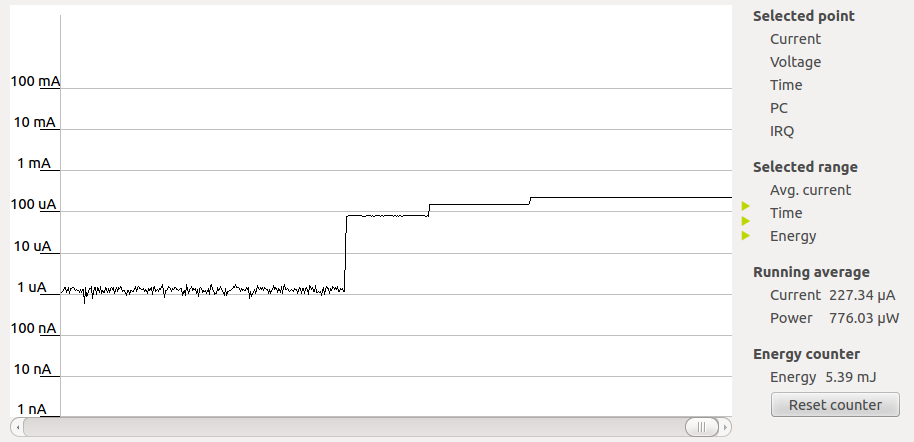
\includegraphics[width=\textwidth]{images/eaprofiler.png}
\caption{A screenshot from the eAProfiler program, showing current when idle and 1, 2 and 3 buttons are depressed.}
\end{figure}
\chapter{Conclusion}
In this assignment we started with making the device driver for the gamepads buttons and figuring out how to draw on the screen, before we starting to implement the core game. 
We successfully implemented the game we intended to based on the original. We learned about making device drivers for Linux, char drivers, the linux framebuffer and the process behind implementing Linux on the development board (toolchain, ptxdist, etc).
\\
Not many issues were encountered except for normal development bumps. Some faulty documentation and guides hampered our progress, but most were fixed by trial and error to get it working. 
\\
The final product is a playable game for two players (or one if you're handy).

Only 4 of the 8 buttons are used for controlling the game, so it may have been possible to make it 4 player by utilizing all 8 buttons for playing instead.  


% Bibliography - edit references.bib and use the \cite command in text
\bibliographystyle{plain}
\bibliography{references}
\end{document}
